
\newpage

\subsection{Functionaliteit van threads}

\noindent $\Rightarrow$ Net zoals processen hebben threads  verschillende uitvoeringstoestanden en kunnen ze met elkaar synchroniseren.

\subsubsection{Thread toestanden (=states)}

\textbf{Er zijn vier basisbewerkingen met threads die samenhangen met een verandering van de threadtoestand:}

\begin{itemize}
    \item Verwekken (Spawn).
        \begin{itemize}
        \item Wanneer er een nieuw proces wordt aangemaakt wordt er meestal een nieuwe thread aangemaakt.
        \end{itemize}
    \item Blokkeren(Block). 
        \begin{itemize}
        \item Als een thread moet wachten op een gebeurtenis wordt deze thread geblokkeerd. De processor schakelt dan over op een andere thread. 
        \item Probleem: Het kan wel zijn dat als je een thread blokkeert een andere thread of alle andere threads ook geblokkeerd zijn.
        \end{itemize} 
    \item Deblokkeren(Unblock). 
        \begin{itemize}
        \item Bij het optreden van de gebeurtenis waarvoor de geblokkeerde thread wacht, wordt deze thread overgebracht naar de toestand Gereed.
        \end{itemize}
    \item Beëindigen(Finish).
        \begin{itemize}
        \item Als een thread voltooid is, worden de registercontext en de stacks van de thread ongedaan gemaakt (deallocate).
        \end{itemize}
\end{itemize}

Stel dat we een programma hebben dat twee maal een externe procedureaanroep (remote procedure call RPC) verzendt naar twee verschillende hosts om een gecombineerd resultaat te verkrijgen. Bij de volgende figuur zie je hoe het zou zijn met één thread:



\begin{figure}[htp]
    \centering
            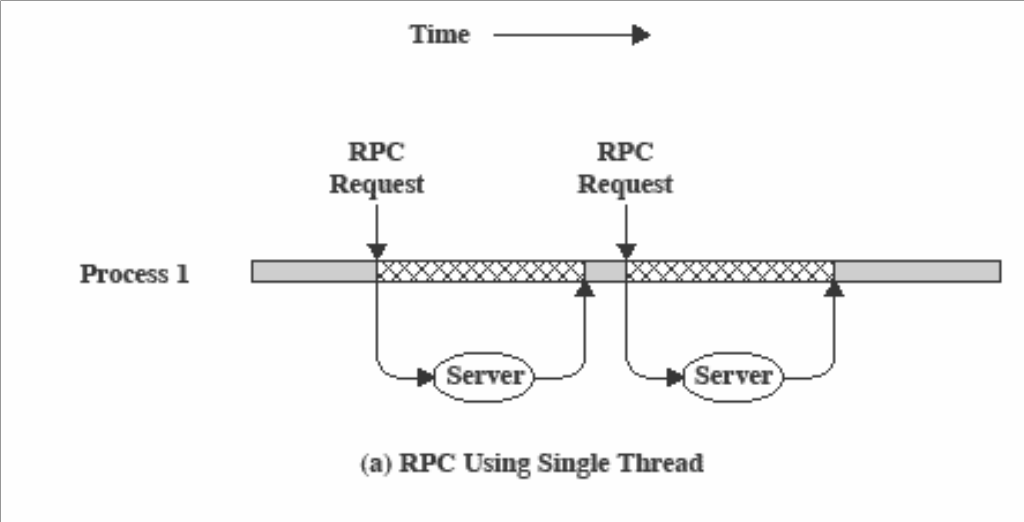
\includegraphics[width=4in]{img/rpcsinglethread.png}
        \caption{RPC Using Single Thread}
    \label{fig:RPC Using Single Thread}
\end{figure}

\newpage

Volgende figuur zie je het geval hoe het zou zijn moest men 1 thread per server gebruiken.

\begin{figure}[htp]
    \centering
            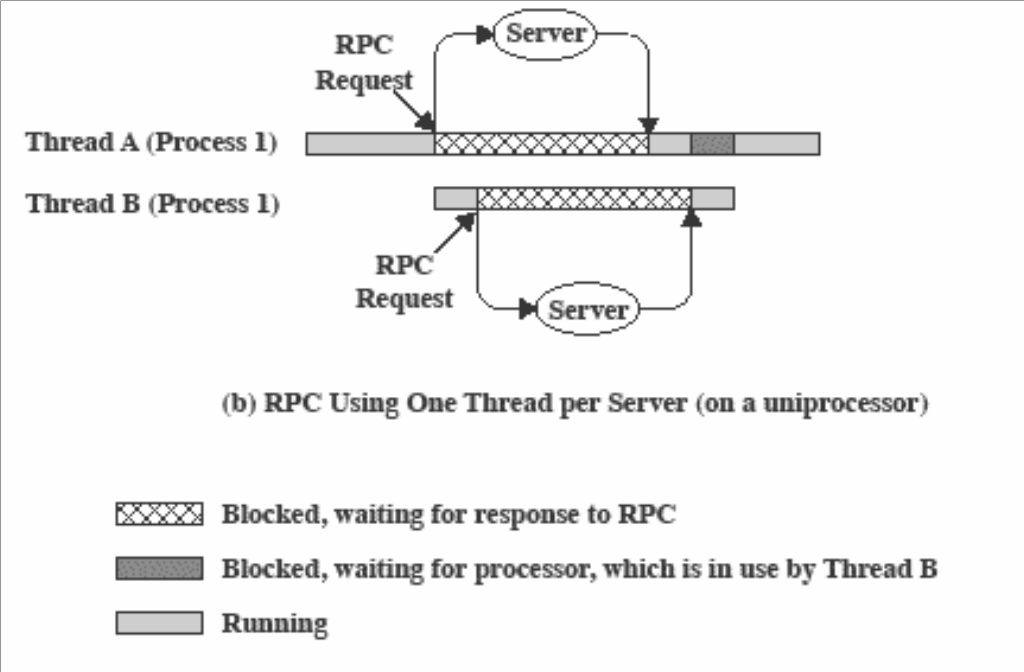
\includegraphics[width=4in]{img/threadperserver.png}
        \caption{1 Thread per server}
    \label{fig:1 Thread per server}
\end{figure}

Bij een uniprocessor maakt multiprogramming het verweven van meerdere threads binnen meerdere processen mogelijk.

\subsubsection{Threads op gebruikersniveau en op kernelniveau}

\textbf{Er bestaan twee algemene vormen voor implementatie van threads:}

\begin{itemize}
\item Threads op gebruikersniveau (ULT User Level Thread)
\item Threads op kernelniveau (KLT Kernel Level Thread)
\end{itemize}

\textbf{Bij User-Level Threads:}

\begin{itemize}
        \item Het threadbeheer wordt gedaan door het programma.
        \item De kernel weet niet van het bestaan van de threads.
\end{itemize}

\newpage

\textbf{De samenhang tussen ULT en de procestoestand (zie meer uitleg boek p 185)}

\begin{figure}[htp]
    \centering
            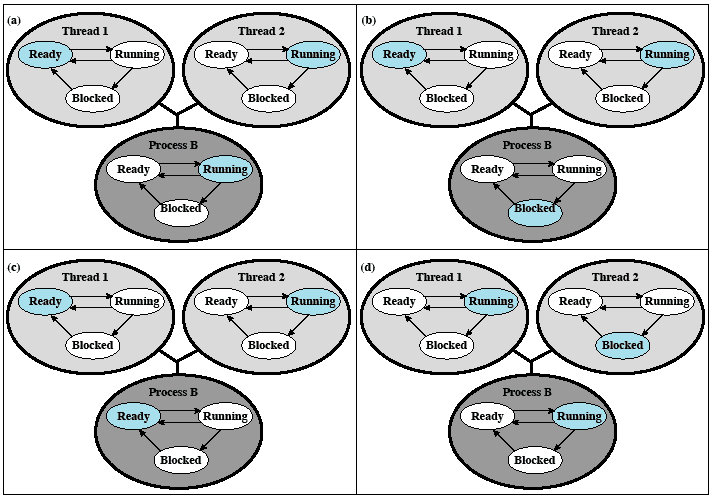
\includegraphics[width=4in]{img/samenhangultprocestoestand.png}
        \caption{Samenhang tussen ULT en de procestoestand}
    \label{fig:Samenhang tussen ULT en de procestoestand}
\end{figure}

\textbf{Bij Kernel-Level Threads:}

\begin{itemize}
    \item De kernel beheert de threads en onderhoudt de contextinformatie voor het proces en de threads.
    \item De scheduling door de kernel wordt gedaan op basis van threads.
        
    \item Windows is een voorbeeld van deze benadering.
\end{itemize}
	
\textbf{Voordelen van Kernel-Level Threads tegenover User-Level Threads:}

\begin{itemize}
    \item De kernel kan meerdere threads van hetzelfde proces schedulen op meerdere processen.
    \item De kernel kan bij een geblokkeerde thread in een proces een andere thread van hetzelfde proces schedulen.
\end{itemize}

\textbf{Nadeel van Kernel-Level Threads tegenover User-Level Threads:}

Er is een moduswisseling nodig naar kernel-mode om de besturing van de ene thread over te dragen naar de andere thread.

\textbf{Gecombineerde benaderingen:}

\begin{itemize}
\item De thread creatie wordt gedaan in de gebruikersruimte, het grootste deel van de scheduling en synchronisatie van threads binnen een toepassing wordt ook gedaan in de gebruikersruimte.
\item Voorbeeld is Solaris.
\end{itemize}

\subsubsection{Andere indelingen}

    \begin{center}
    \def\arraystretch{1.5}%  1 is the default, change whatever you need

    \begin{tabular}{ | p{4cm} | p{6cm} | p{5cm} |}
    \hline
    Threads : processen & Beschrijving & Voorbeeldsystemen \\ \hline
    1:1 (één op één)     & Elke uitvoeringsthread is een uniek proces met een eigen adresruimte en eigen bronnen. & Dit was de oorspronkelijke implementatie van UNIX \\ \hline
   M : 1 (veel op één)   & Een proces definieert een adresruimte en dynamische bezit van bronnen. Binnen het proces kunnen meerdere threads worden gecreëerd en uitgevoerd. & Windows NT, Solaris, Linux OS/2, OS/390, MACH \\ \hline
1 : M (één op veel)      & Een thread kan migreren van de ene naar de andere procesomgeving. Hierdoor kan een thread eenvoudig worden verplaatst tussen verschillende systemen. & RA(Clouds), Emeralds \\ \hline
   M : N (veel op veel)  & Combineert de eigenschappen van M : 1 en 1 : M & TRIX \\ \hline
    \end{tabular}
\end{center}

